\documentclass[12pt]{article}
\usepackage[top=1in, bottom=1in, left=.75in, right=.75in]{geometry}
\usepackage{amsmath}
\usepackage{fancyhdr}
\usepackage{graphicx}
\usepackage{txfonts}
\usepackage{multicol,coordsys}
\usepackage[scaled=0.86]{helvet}
\renewcommand{\emph}[1]{\textsf{\textbf{#1}}}
\usepackage{anyfontsize}
% \usepackage{times}
% \usepackage[lf]{MinionPro}
\usepackage{tikz,pgfplots,mathrsfs}
%\def\degC{{}^\circ{\rm C}}
\def\ra{\rightarrow}
\usetikzlibrary{calc}
\pgfplotsset{compat = newest}
\newcommand{\blank}[1]{\rule{#1}{0.75pt}}

\pgfplotsset{my style/.append style={axis x line=middle, axis y line=
middle, xlabel={$x$}, ylabel={$y$},axis equal}}

%yticklabels={,,} , xticklabels={,,}

% \setmainfont{Times}
% \def\sansfont{Lucida Grande Bold}
\parindent 0pt
\parskip 4pt
\pagestyle{fancy}
\fancyfoot[C]{\emph{\thepage}}
\fancyhead[L]{\ifnum \value{page} > 1\relax\emph{Math 251: Midterm 1}\fi}
\fancyhead[R]{\ifnum \value{page} > 1\relax\emph{April 7, 2022}\fi}
\headheight 15pt
\renewcommand{\headrulewidth}{0pt}
\renewcommand{\footrulewidth}{0pt}
\let\ds\displaystyle
\def\continued{{\emph {Continued....}}}
\def\continuing{{\emph {Problem \arabic{probcount} continued....}}\par\vskip 4pt}


\newcounter{probcount}
\newcounter{subprobcount}
\newcommand{\thesubproblem}{\emph{\alph{subprobcount}.}}
\def\problem#1{\setcounter{subprobcount}{0}%
\addtocounter{probcount}{1}{\emph{\arabic{probcount}.\hskip 1em(#1)}}\par}
\def\subproblem#1{\par\hangindent=1em\hangafter=0{%
\addtocounter{subprobcount}{1}\thesubproblem\emph{#1}\hskip 1em}}
\def\probskip{\vskip 10pt}
\def\medprobskip{\vskip 2in}
\def\subprobskip{\vskip 45pt}
\def\bigprobskip{\vskip 4in}

\begin{document}
{\emph{\fontsize{26}{28}\selectfont Math F251\hfill
{\fontsize{32}{36}\selectfont Midterm 2}
\hfill Spring 2022}}
\vskip 2cm
\strut\vtop{\halign{\emph#\hskip 0.5em\hfil&#\hbox to 2in{\hrulefill}\cr
\emph{\fontsize{18}{22}\selectfont Name:}&\cr
\noalign{\vskip 10pt}
%\emph{\fontsize{18}{22}\selectfont Student Id:}&\cr
%\noalign{\vskip 10pt}
%\emph{\fontsize{18}{22}\selectfont Calculator Model:}&\cr
}}
\hfill
\vtop{\halign{\emph{\fontsize{18}{22}\selectfont #}\hfil& \emph{\fontsize{18}{22}\selectfont\hskip 0.5ex $\square$ #}\hfil\cr
Section: & 001 (Jill Faudree)\cr
\noalign{\vskip 4pt}
         & 002 (James Gossell)\cr
\noalign{\vskip 4pt}
         & 005 (James Gossell)\cr}}

\vfill
{\fontsize{18}{22}\selectfont\emph{Rules:}}

You have 60 minutes to complete the exam.  

Partial credit will be awarded, but you must show your work.

The exam is closed book and closed notes.

Calculators are not allowed. 


Place a box around your  \fbox{FINAL ANSWER} to each question where appropriate.

%If you need extra space, you can use the back sides of the pages.
%Please make it obvious  when you have done so.

Turn off anything that might go beep during the exam.

Good luck!
\vfill
\def\emptybox{\hbox to 2em{\vrule height 16pt depth 8pt width 0pt\hfil}}
\def\tline{\noalign{\hrule}}
\centerline{\vbox{\offinterlineskip
{
\bf\sf\fontsize{18pt}{22pt}\selectfont
\hrule
\halign{
\vrule#&\strut\quad\hfil#\hfil\quad&\vrule#&\quad\hfil#\hfil\quad
&\vrule#&\quad\hfil#\hfil\quad&\vrule#\cr
height 3pt&\omit&&\omit&&\omit&\cr
&Problem&&Possible&&Score&\cr\tline
height 3pt&\omit&&\omit&&\omit&\cr
&1&&12&&\emptybox&\cr\tline
&2&&10&&\emptybox&\cr\tline
&3&&10&&\emptybox&\cr\tline
&4&&10&&\emptybox&\cr\tline
&5&&10&&\emptybox&\cr\tline
&6&&10&&\emptybox&\cr\tline
&7&&16&&\emptybox&\cr\tline
&8&&12&&\emptybox&\cr\tline
&9&&10&&\emptybox&\cr\tline
&Extra Credit&&5&&\emptybox&\cr\tline
&Total&&100&&\emptybox&\cr
}\hrule}}}

\newpage
\begin{enumerate}
%sketching
\item (12 points) Sketch graphs which satisfy the given conditions. \textbf{There are many correct answers.}
	\begin{multicols}{2}
	\begin{enumerate}
	\item Sketch a graph of a function $f(x)$ that has
		\begin{itemize}
		\item a local maximum at $x=-5$, and
		\item a local minimum at $x=5$.
		\end{itemize}
	\begin{center}
	\rescaleby{1}{10}{\vlabel}
	\rescaleby{1}{10}{\hlabel}
	\coordsys[10][10](-75,-75)(75,75)
	\end{center}
	
	\item Sketch a graph of a function $k(x)$ that has
		\begin{itemize}
		%\item an inflection point at $x=5$
		\item $k''(x) < 0$ for $x<5$, and
		\item $k''(x) > 0$ for $x>5$.
		\end{itemize}
	\begin{center}
	\rescaleby{1}{10}{\vlabel}
	\rescaleby{1}{10}{\hlabel}
	\coordsys[10][10](-75,-75)(75,75)
	\end{center}

	
\columnbreak
\item Sketch a graph of a function $g(x)$ such that
		\begin{itemize}
		\item $\displaystyle \lim_{x \to -\infty} $g(x)$ = 2$, and
		\item $\displaystyle \lim_{x \to \infty} $g(x)$ = -2$.
		\end{itemize}
	\begin{center}
	\rescaleby{1}{10}{\vlabel}
	\rescaleby{1}{10}{\hlabel}
	\coordsys[10][10](-75,-75)(75,75)
	\end{center}

	\item Sketch a graph of a function $h(x)$ such that
		\begin{itemize}
		\item $h'(5)>0$, and
		\item $h''(5)<0$.
		\end{itemize}
	\begin{center}
	\rescaleby{1}{10}{\vlabel}
	\rescaleby{1}{10}{\hlabel}
	\coordsys[10][10](-75,-75)(75,75)
	\end{center}

	

	\end{enumerate}
	\end{multicols}


\pagebreak

%lhopitals
\item (10 points) Evaluate the following limits. You must show your work to earn full credit. If you apply L'Hopital's Rule, you should indicate this.
	\begin{enumerate}
	\item $\displaystyle{\lim_{x\to 1} \frac{4x^2-8x+4}{-x^4+x^3+x^2-x}}$
	\vspace{1.5in}
	\item $\displaystyle{\lim_{x\to 0} \frac{x\cos 3x}{\sin 3x}}$
	\vspace{1.5in}
	\end{enumerate}
	
%linear approximation
\item (10 points) 
	\begin{enumerate}
	\item Find the linear approximation (also known as the linearization) of the function $f(x)=x^3$ when $a=2.$
	\vfill
	\item Use the linear approximation to estimate $(2.02)^3$. Your answer must be in the form of a decimal.
	\vfill
	\end{enumerate}
\newpage

%related rate
\item (10 points) \textbf{[Related Rates Problem]} A hiker and a baby bear meet in the woods. Both are terrified! The hiker runs west at $3$ meters per second. The bear lumbers south at $4$ meters per second.
	\begin{enumerate}
	\item Draw a diagram.
	\vspace{2in}
	\item Determine how fast the distance between the hiker and bear is 	increasing  $2$ seconds after the hiker and baby bear meet. Include units with your answer.
	\vspace{2in}
	\end{enumerate}
\newpage
%Abs. Max and Min / Closed interval method
\item (10 points) 
	\begin{enumerate}
	\item Find all critical values of $\displaystyle{f(x)=\frac{x^2+2}{2x+1}}$ on the interval $[0,4]$.
	\vfill
	\item Identify the absolute maximum and absolute minimum of the function $f(x)$ on the interval $[0,4].$
%Test the critical values and the endpoints $x=0$ and $x=4$ to find the absolute maximum and absolute minimum of $f(x)$ on $[0,4]$.\\
	\vfill

	\textbf{Absolute max:}  $y=$\hspace{2.5in} \textbf{Absolute min:} $y=$
	\end{enumerate}

\pagebreak



%Max/min problem
\item (10 points) \textbf{[Optimization Problem]} Find the two \textbf{positive} numbers $x$ and $y$ on the circle $x^2 + y^2 = 48$ that maximize the product $P=xy^2.$ \\
Note: Your solutions must use Calculus to \emph{justify} that your answer is correct.\\
\vfill
%Follow the steps below to find the two positive numbers $x$ and $y$ on the circle $x^2 + y^2 = 18$ that maximize the product $P=xy$?
%\begin{enumerate}[a.]
%\item Solve the equation $x^2 + y^2 = 18$ for $y$.
%\vspace{1in}
%\item Replace $y$ in the objective function $P=xy$ with the expression you got in part a.
%\vspace{1in}
%\item Take the derivative of $P$ with respect to $x$ to find the critical values of $P$.
%\vspace{2in}
%\item Determine which $x$-value maximizes the product. Then solve for $y$ as well.
%\vspace{2in}

\textbf{x =} \hspace{1in} \textbf{y=}
%\end{enumerate}

\newpage
%derivative + shape of graph
\item (16 points) Use the information below to answer questions about the function $f(x).$ You must show your work to earn full credit. \\
$$f(x)=x^{4/3}-4x^{1/3}, \hspace{.2in} f'(x)=\frac{4x-4}{3x^{2/3}},
\hspace{.2in} f''(x)=\frac{4x+8}{9x^{5/3}}.$$

\begin{enumerate}
\item  Determine the intervals on which $f(x)$ is increasing/decreasing.
\vfill
\item Find the $x$-values that correspond to any local maximums or local minimus of $f(x)$. 
\vfill
\item Find the intervals on which $f(x)$ is concave up and concave down.
\vfill 
\item Find the $x$-values of any inflection points of $f(x).$ If there aren't any, you must explicitly state this and justify your answer.
\vfill
\end{enumerate}

\newpage

%area under curve
\item (12 points) 
\begin{enumerate}
\item Estimate the area under the curve $f(x)=\ln(x)$ on the interval $[1,9]$ using $R_4.$ (That is, use 4 approximating rectangles and right-hand end points.) Sketch the approximating rectangles on the graph below.\\
Note: You are obviously not expected to compute things like $\ln(3)$. It is acceptable to have numbers like this in your final answer.\\

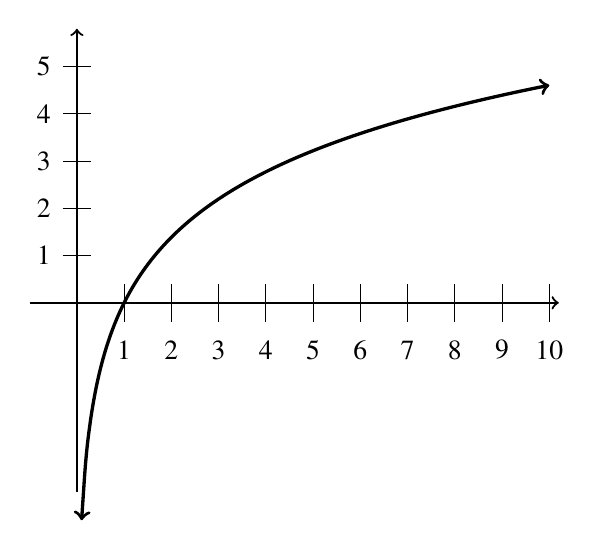
\begin{tikzpicture}[scale=.6]
\draw[thick, ->] (0,-4) -- (0,5.8);
\draw[thick, ->] (-1,0) -- (10.2,0);
\foreach \i in {1,2,3,4,5,6,7,8,9,10}{
	\draw (\i,-0.4) -- (\i, 0.4);
	\node at (\i,-1){$\i$};
	}
\foreach \i in {1,2,3,4,5}{
	\draw (-0.3,\i) -- (0.3,\i);
	\node at (-0.7,\i){$\i$};
	}
%\draw (-.5,5) -- (0.5,5);
%\node at (-1,5.2){5};
%\draw[ultra thick] (-2,0)--(2,0) -- (2, 3.666) -- (-2,3.666) -- (-2,0);
%\node[draw, circle, fill=black,scale=0.4] at (2,3.666){};
%\node at (3,4){$(x,y)$};
%\draw[black, line width = 0.40mm]   plot[smooth,domain=0.5:10] (\x, ln(\x));
\draw[<->,line width=1.2pt,smooth,samples=100,domain=0.1:10] plot(\x,{2*ln((\x))});
\end{tikzpicture}
\vfill
\item In fact, the area under the graph $f(x)$ on the interval $[1,9]$ about $11.8$. Use this fact to evaluate the definite integrals below:
	\begin{enumerate}
	\item $\displaystyle \int_1^9 2 \ln(x) \: dx=$
	\vfill
	\item $\displaystyle \int_1^9 2+ \ln(x) \: dx=$
	\vfill
	\end{enumerate}
\end{enumerate}
\newpage
%antiderivatives
\item (10 points) Evaluate the indefinite integrals below. 
	\begin{enumerate}
	\item $ \displaystyle \int (4\cos(x)+x^{2.3} + 10) \: dx$
	\vfill
	\item $ \displaystyle \int (x^2+4)^2 \: dx $
	\vfill
%	\item $ \displaystyle \int \left(\frac{1}{1+x^2}+\frac{1+x^2}{x} \right) \: dx$
%	\vfill
	\end{enumerate}
%%horizontal asymptotes
%\item (6 points) A population of deer is modeled by the equation below where $P$ is the number of deer and $t$ is time in years.
%$$P(t)=\frac{1500e^t}{7+3e^t}$$
%\begin{enumerate}
%	\item Determine $\displaystyle \lim_{t \to \infty} P(t).$ 
%	\vfill
%	\item What does your answer in part (a) indicate about the graph of $P(t)$?
%	\vfill
%	\item Interpret your answer in part (a) in the context of the problem.
%	\vfill
%\end{enumerate}
%\newpage



%%interpretation of area under curve
%\item (6 points) Oil leaked from a tank at a rate of $r(t)$ liters per hour. The rate decreased as time passed and values of the rate at 3-hour intervals are shown in the table below. Estimate the total amount of oil that leaked from the tank in the 12 hour period. Include units with your anwer.\\
%
%\begin{tabular}{l | c|c|c|c|c}
%$t$ (in hours)& 0&3&6&9&12\\
%\hline
%$r(t)$ (in liters/hour)\quad \quad &9&8&6&4&1\\
%\end{tabular}
%

\end{enumerate}

\textbf{Extra Credit (5 points):} The function $\displaystyle P(t)=\frac{5e^t}{e^t+2}$ models a population of caribou (in hundreds) over time $t$ in years. Evaluate the $\displaystyle \lim_{x \to \infty} P(t)$ and interpret the answer in the context of the problem. (Your interpretation should be a complete sentence that a regular person can understand.)

%According to this model, at what time is the population of caribou growing the fastest?\\
%
%Note that $\displaystyle P'(t)=\frac{10e^t}{(2+e^t)^2}$ and $\displaystyle P''(t)=\frac{-10e^t(e^t-2)}{(2+e^t)^3}.$


\vspace{4in}
\end{document}
